\documentclass[10pt,conference,compsocconf]{IEEEtran}

%\usepackage{times}
%\usepackage{balance}
\usepackage{url}
\usepackage{graphicx}	% For figure environment


\begin{document}
\title{Writing Scientific Papers and Software}

\author{
  David Chettrit\\
  Stephan Seebacher\\
  Sezer Gueler\\
  Department of Computer Science, ETH Zurich, Switzerland
}

\bibliographystyle{plain}
\bibliography{howto-paper.bib}

\maketitle

\begin{abstract}

\end{abstract}

\section{Introduction}



\section{The Structure of a Paper}
\label{sec:structure-paper}



\section{Neural Networks}
\label{sec:tips-writing}

\subsection{Neural Networks}
Inspired by biological nervous systems, such as the human brain, artificial neural networks are used for information processing. In biological nervous systems, highly interconnected neurons work together to solve a specific task. Each neuron solves a subtask and communicates with other neurons. In artificial neural networks this idea is used to approximate arbitrary  non-linear functions. The nodes(neurons) are connected by weighted edges and the topology is chosen depending on the problem. In the training phase, the weights of the edges are set depending on the data. Neural networks are often represented in layers. Each layer contains some of the nodes and then follows the interconnections and then the next layer. 
\\
wieso verwendet man denn gerade Neuronale netzwerke....
\subsection{Neural Network Structure}
\begin{figure}[tbp]
  \centering
  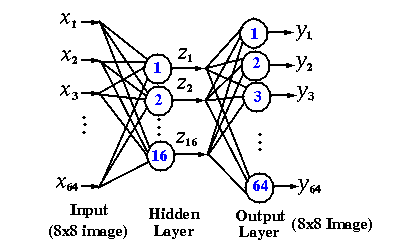
\includegraphics[width=\columnwidth]{nnStructure}
  \caption{Neural Network Structure for compression.}
  \label{fig:nnStructure}
\end{figure}

Figure~\ref{fig:nnStructure} shows the neural network structure we use for compression. There are three layers: input layer, hidden layer and output layer. The input layer and the hidden layer are fully interconnected as are the hidden layer and the output layer. The weights of the edges are detrermined by the training algorithm which is described in the next section. 

\subsection{Neural Network Training Algorithm}
-Levenberg-Marquardt

\subsection{Singular Value Decomposition}
The singular value decomposition(SVD) is a matrix factorization. A m$\times$n matrix M can be written as a product of three matrices U, $\Sigma$ and V$^*$, where U is a unitary m$\times$m matrix, V$^*$ is the conjugate transpose of a n$\times$n unitary matrix V and $\Sigma$ is a m$\times$n diagonal matrix. The entries on the diagonal of $\Sigma$, which are non-negativ real numbers, are called the singular values of M. \\
SVD can be used for image compression the following way. The singular values are sorted in descending order and then only the largest singular values and the corresponding right and left singular vectors are used to save the image.
\subsection{Models and Methods}


\subsection{Results}


\section{Tips for Good Software}
\label{sec:tips-software}



\section{Computational Intelligence Laboratory Requirements}
\label{sec:cil}
\subsection{Developing a Novel Solution}

\subsection{Comparison to Baselines}

\subsection{Write Up}



\subsubsection{Installation}

\subsubsection{Compiling \LaTeX{}}

\subsubsection{Equations}

\subsubsection{Tables and Figures}

\subsection{Grading}

\section{Summary}

\section*{Acknowledgements}


\bibliographystyle{IEEEtran}
\bibliography{howto-paper}
\end{document}
